%https://tex.stackexchange.com/questions/208819/embedding-images-in-tex-file-as-base64-strings

%Questo è il preambolo, dove si inseriscono i pacchetti e le impostazioni che servono per compilare il documento. Quanto scritto dopo il simbolo '%' è solo un commento e serve a fini dimostrativi.
\documentclass{article}
%\documentclass[a4paper, 13pt, oneside]{report}
\linespread{1.5} %interlinea
\pagestyle{plain}
\usepackage{chngpage}

\usepackage{geometry} %margini
\geometry{a4paper, top=3cm, bottom=3cm, left=3cm, right=3cm, bindingoffset=5mm}
\usepackage{graphicx}
\usepackage{siunitx}
\usepackage{subcaption}
\graphicspath{img/}
\usepackage{multicol} %più colonne
\usepackage{ragged2e} %allineamento testo

% italian is gay
%\usepackage[italian]{babel} %lingua principale

\usepackage{minitoc} %mini sommario a inizio capitolo
\nomtcrule





\usepackage{comment}








\usepackage{xpatch}
\usepackage{blindtext}


\makeatletter

\makeatother

\usepackage{fancyhdr}
\usepackage[export]{adjustbox}



\usepackage{hyperref} %hyperlink
\hypersetup{
    colorlinks=true,
    citecolor=cyan,
    linkcolor=black,
    urlcolor=black,
    pdftitle=Report - {\VAR{name}},
    pdfauthor=Un povero studente di medicina,
    }

\usepackage{booktabs} %per le tabelle
\usepackage{multirow}
\usepackage[table,xcdraw]{xcolor}
\usepackage{graphicx}

\usepackage{lscape}
\usepackage{float}
\usepackage{wrapfig}

%Da qui in poi inizia il documento.
\begin{document}
\begin{titlepage} %Cambia i valori in \vspace{} per ottenere un risultato perfetto

\begin{center}
	{\scshape\Large\bfseries \, \par}
	\vspace{5cm}


	
\includegraphics{/app/img/Provins.png}\par



	\vspace{0,5cm}
	{\scshape\Large\bfseries Recommended Asset Allocation

	{\VAR{name}} | 11/20/2020 \par}
	\vspace{0,5cm}
	{\scshape\normalsize Frontier Curve Optimal Portfolio Analysis

	Monte Carlo Simulation Of Returns

	Correlation Matrix \par}
\end{center}

	\begin{center}
\line(1,0){250}
\end{center}

	\begin{center}
	 	{
		\small{
		Prepared by Thomas K. Provins

		THOMAS.PROVINS@LPL.COM}
		\par}


	\vfill
\end{center}

	\vfill

% Bottom of the page
	{\begin{center}

	     1910 Cochran Road

	     Manor Oak 2 Suite 450

	     412.440.6949

	\end{center}}

\end{titlepage}


\tableofcontents

\begin{center}
\vfill
\vfill

\end{center}
\justify

\newpage

\section{Statistical Terminology \& Asset Class Descriptions}

\textbf{Expected Return} - Of an investing strategy is the amount of money you are expected to get back from your investment. For example, if 90 dollars is invested for 1 year with an expected return of 100 dollars, then in the average case the investment will yield back 100 dollars.


\vspace{.5cm}

\noindent \textbf{Risk} - Or standard deviation of an investing strategy is a measure of how much the return of an investment strategy will vary from it's expected return. For example, an investment strategy with an expected return of 20\% and a risk of 8\% will yield 112\% to 128\% return with a probability of 68.2\% , and 104\% to 136\% return with a probability of 94.4\%

\vspace{1cm}
\large
\noindent \textbf{The 18 Asset Classes : }
\normalsize
\vspace{.5cm}
\begin{adjustwidth}{0in}{0in}% adjust the L and R margins by 1 inch
\begin{tabular}{lll} %\toprule
    Asset Class & Index & Description\\ \midrule

    Large Cap Growth  & FSPGX & Fastly growing stocks from big companies. \\\midrule
    Large Cap Value & SVX & Undervalued stocks from big companies. \\\midrule
    Small Cap Growth & RUT & Fastly growing stocks from small companies.\\\midrule

    Small Cap Value  & RUJ & Undervalued stocks from small companies. \\\midrule
    Mid Cap  & SP400 & Stocks from mid sized companies. \\\midrule
    International  & VTIAX & Stocks not traded in U.S.A. exchanges. \\\midrule

    Emerging Mkt.  & VEMAX & Stocks from emerging Mkt. countries. \\\midrule
    Real Estate  & DJUSRE & Land and buildings. \\\midrule
    Venture Capital  & AMZX &  New and innovative companies. \\\midrule

Inter. Govt. Bonds  & GVI & Govt. bonds that mature in 5-10 years. \\\midrule
    Long Govt. Bonds  & ILTB & Govt. bonds mature in more than 10 years. \\\midrule

    Corporate Bonds  & SPDBDACPT & Bonds issued by a corporation. \\\midrule
    High Yield Bond  &HYG & Lower credit rating higher return bonds. \\\midrule
    Municipal Bond  & MUB & Bonds Issued by local government. \\\midrule

    Foreign Bonds  & BNDX & Bonds issued in other countries. \\\midrule
    Emerging Mkt. Debt  & JEDAX & Bonds issued by emerging countries. \\\midrule
    Commodities  & DJCI & Basic goods used in commerce.
\\\midrule

    Cash  & BIL & Currencies, Foreign Currencies

    \\ \bottomrule
\end{tabular}
\end{adjustwidth}


\newpage

\section{Investment Profile | Prescribed Allocation Changes}

\vspace{.5cm}
\begin{tabular}{lr}
\begin{tabular}[t]{l}
\vspace{.1cm}\\
\large\textbf{\underline {Investment Profile:}}
\vspace{.25cm}\\
\noindent Name : {\VAR{name}} \\
\noindent Birthday : 11/20/1960 \\
%\noindent Purpose : Retirement \\
\noindent Time Frame : 9 Years \\
\noindent Available Funds : \$1,232,683.45 \\
\noindent Preferred Risk : ($\pm 8\%$ Yearly) \\
\noindent \textbf{Preffered Asset Classes:} \\
- Large Cap Growth Stocks\\
- Large Cap Value Stocks\\
- High Yield Bonds \\
- Emerging Mkt. Stocks\\
- Venture Capital\\
- Cash\\
\end{tabular} &
\begin{tabular}[t]{c}
(a) Current Portfolio\\
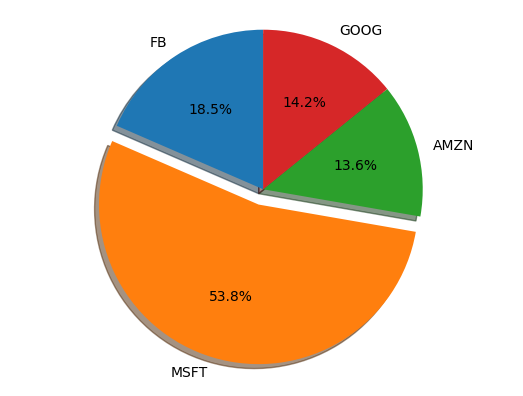
\includegraphics[width=.45\linewidth]{/app/plts/pie.png}\\
(b) New Portfolio\\
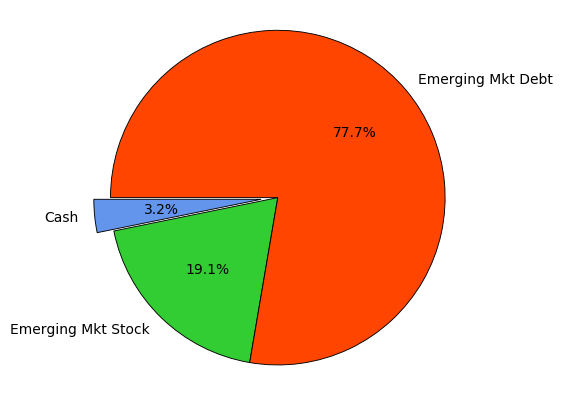
\includegraphics[width=.45\linewidth]{/app/plts/piefuture.png}
\end{tabular}
\end{tabular}

\vspace{.5cm}

\begin{center}
\noindent \large \textbf{\underline{Prescribed Allocation Changes}}\\
\vspace{.5cm}

\normalsize

\begin{tabular}{cccc}
    Asset Class & Current& Suggested & Change\\ \midrule

    Large Cap Growth  & \$54,441.73 & \$43,210.22 & +\$34,321.34 \\\midrule
    Large Cap Value & \$54,441.73 & \$43,210.22 & +\$34,321.34 \\\midrule
    Small Cap Growth & \$54,441.73 & \$43,210.22 & +\$34,321.34 \\\midrule
    Small Cap Value  & \$54,441.73 & \$43,210.22 & +\$34,321.34 \\\midrule
    Mid Cap  & \$54,441.73 & \$43,210.22 & +\$34,321.34 \\\midrule
    International Stock  & \$54,441.73 & \$43,210.22 & +\$34,321.34 \\\midrule

    Emerging Mkt Stock  & \$54,441.73 & \$43,210.22 & +\$34,321.34 \\\midrule

    Real Estate  & \$54,441.73 & \$43,210.22 & +\$34,321.34 \\\midrule
    Venture Capital  & \$54,441.73 & \$43,210.22 & +\$34,321.34
    \\ \bottomrule
\end{tabular}
\end{center}

%1. Large Cap Growth Stocks - Over invested by \$34,323.34. \\
%\,\,\,\,\,\, Reduce your holdings (\$56,372.43$).\\



\newpage

\section{Performance Improvements Of Prescribed Portfolio}

Below are 7 year simulation results of your current investing strategy versus the investment strategy prescribed in this report. \\
Change In Expected Return : \$124,432.23\\
Change in Risk : ( $- 3\%$ )

\vspace{.4cm}
\begin{center}

% OVERLAY BELL AND BELL7 AND LINE AND LINE7 -- generated from MATPLOTLIB as explicit images

\hspace*{-1cm}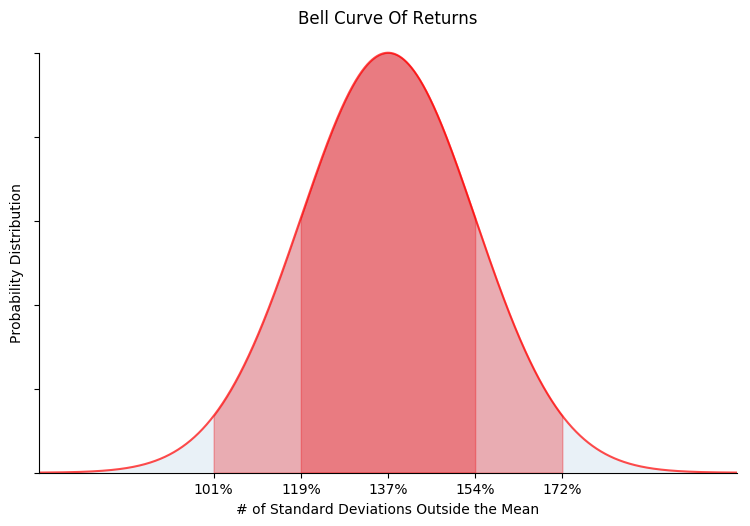
\includegraphics[width=.95\linewidth]{/app/plts/bell.png}\par

\vspace{.5cm}

\hspace*{-1cm}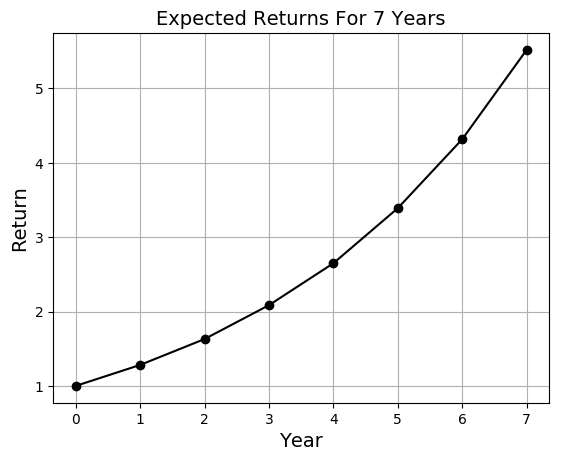
\includegraphics[width=.8\linewidth]{/app/plts/line.png}\par
\end{center}

\newpage

\section{Current Portfolio Overview - Statistical Analysis}

\vspace{1.5cm}

%https://tex.stackexchange.com/questions/257337/how-to-have-a-figure-with-multiple-groups-of-image-and-each-image-with-individua

\begin{adjustwidth}{-.3in}{0in}% adjust the L and R margins by 1 inch
\vspace*{-1cm}

\begin{center}
  \begin{tabular}{c}
    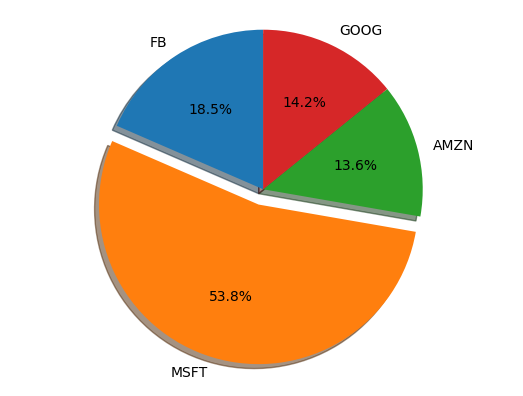
\includegraphics[width=.5\linewidth]{/app/plts/pie.png}
  \end{tabular}
  \end{center}

  \begin{center}
        Portfolio Breakdown
      %(b) Projected Returns (Monte Carlo)
  \end{center}

\vspace{.7cm}


\begin{center}
  \begin{tabular}{lcr}
  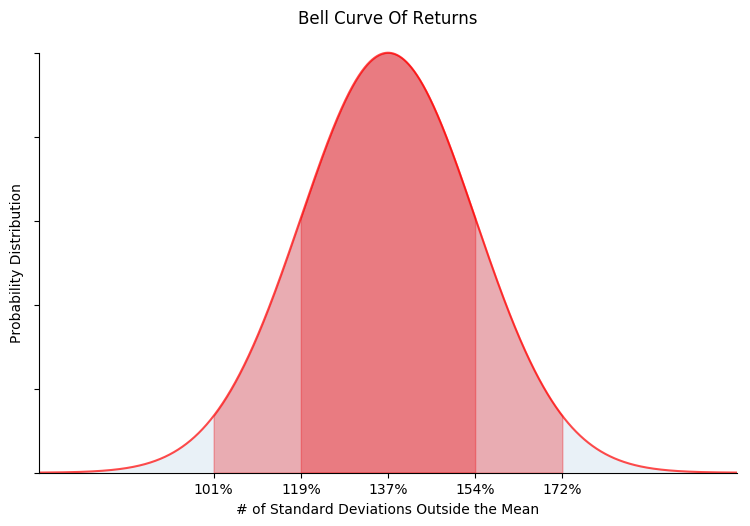
\includegraphics[width=.35\linewidth]{/app/plts/bell.png}
    & \hspace{1cm }&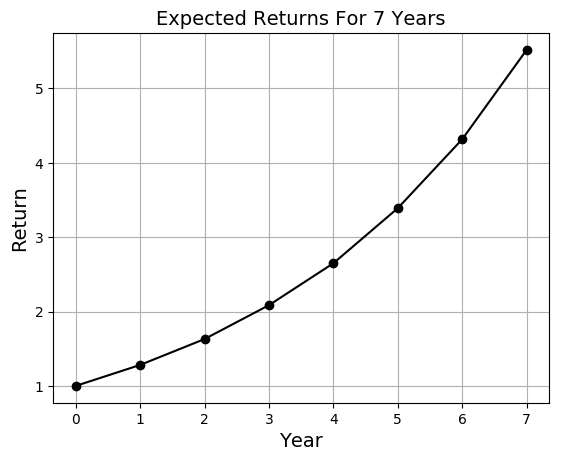
\includegraphics[width=.35\linewidth]{/app/plts/line.png}
  \end{tabular}
  \end{center}

  \begin{center}
      Current Portfolio 1 Year Projections
      %(a) Returns of Current Portfolio
      %(a) Bell Curves Of Expected Return
  \end{center}

  \vspace{.7cm}


\begin{center}
  \begin{tabular}{lcr}
  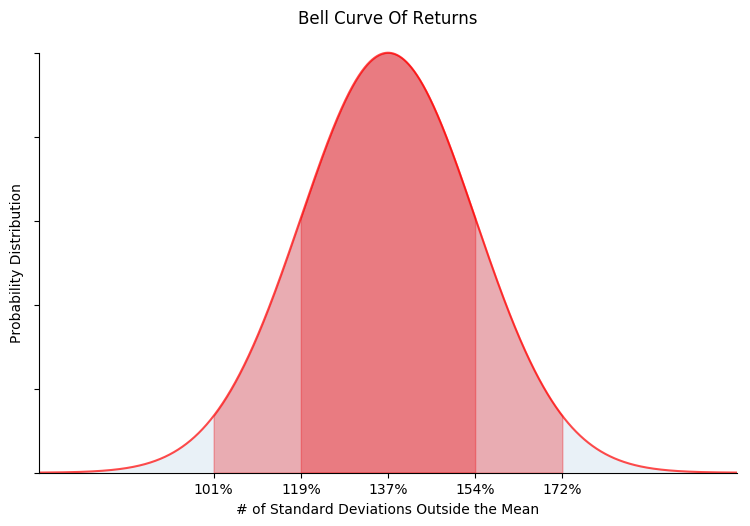
\includegraphics[width=.35\linewidth]{/app/plts/bell.png}
    & \hspace{1cm }&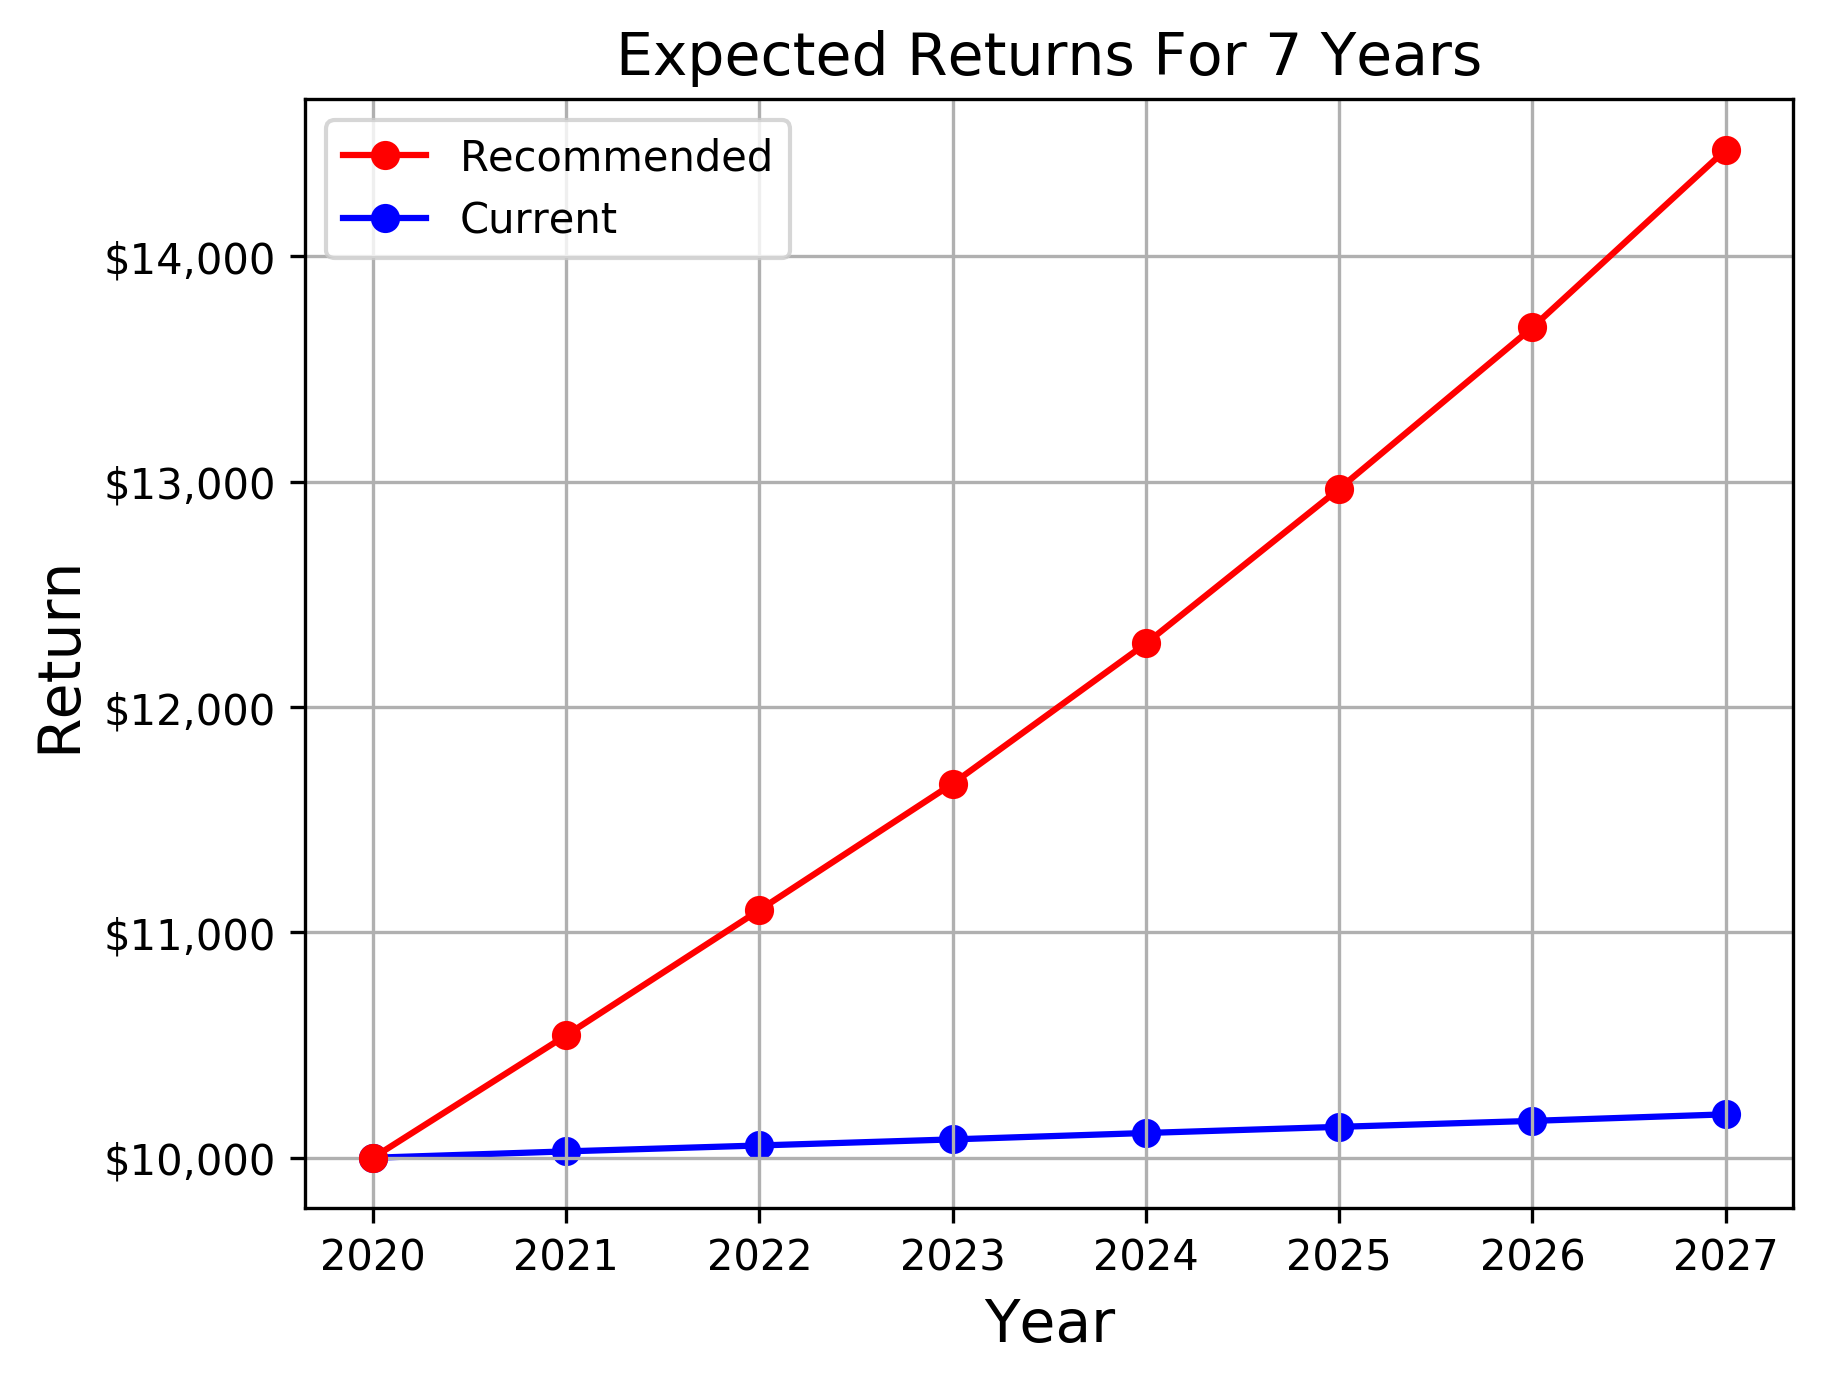
\includegraphics[width=.35\linewidth]{/app/plts/line7.png}
  \end{tabular}
  \end{center}

  \begin{center}
      Current Portfolio 7 Year Projections
      %(a) Returns of Current Portfolio
      %(a) Bell Curves Of Expected Return
  \end{center}

 \vspace{.6cm}

\end{adjustwidth}

\noindent
1 Year Expected Return (\$) : \$343,203.20 (33.3\%)\\
1 Year Risk (Standard Deviation \%) : $\pm$ 3.54\%

\noindent
7 Year Expected Return (\$) : \$343,203.20 (33.3\%)\\
7 Year Risk (Standard Deviation \%) : $\pm$ 3.54\%

\noindent
Sharpe Ratio : .37

\newpage


\section{Prescribed Portfolio Overview - Statistical Analysis}

\vspace{1.5cm}

%https://tex.stackexchange.com/questions/257337/how-to-have-a-figure-with-multiple-groups-of-image-and-each-image-with-individua

\begin{adjustwidth}{-.3in}{0in}% adjust the L and R margins by 1 inch
\vspace*{-1cm}

\begin{center}
  \begin{tabular}{c}
    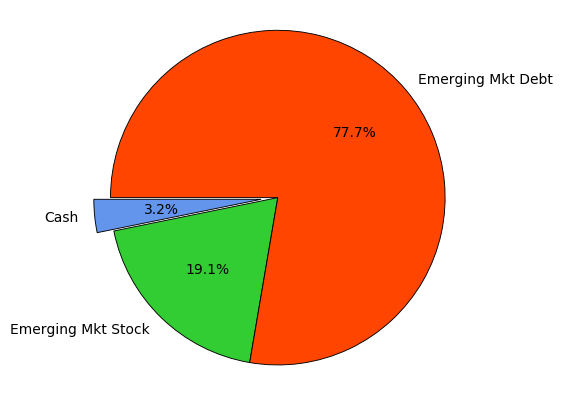
\includegraphics[width=.5\linewidth]{/app/plts/piefuture.png}
  \end{tabular}
  \end{center}

  \begin{center}
        Portfolio Breakdown
      %(b) Projected Returns (Monte Carlo)
  \end{center}

\vspace{.7cm}


\begin{center}
  \begin{tabular}{lcr}
  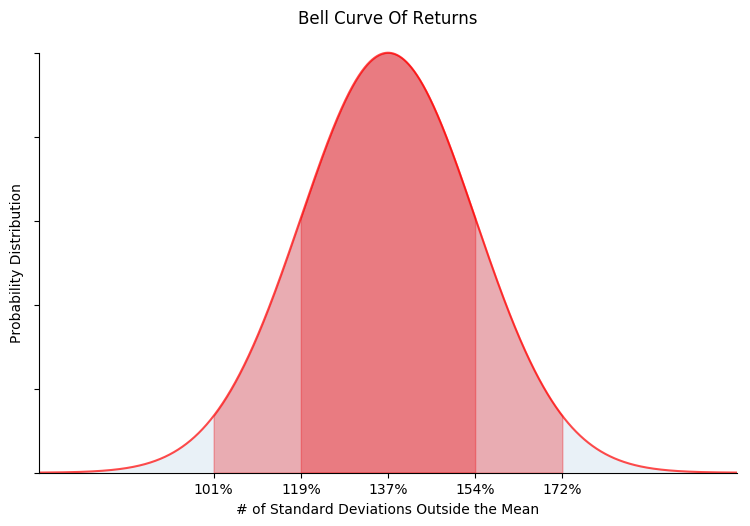
\includegraphics[width=.35\linewidth]{/app/plts/bell.png}
    & \hspace{1cm }&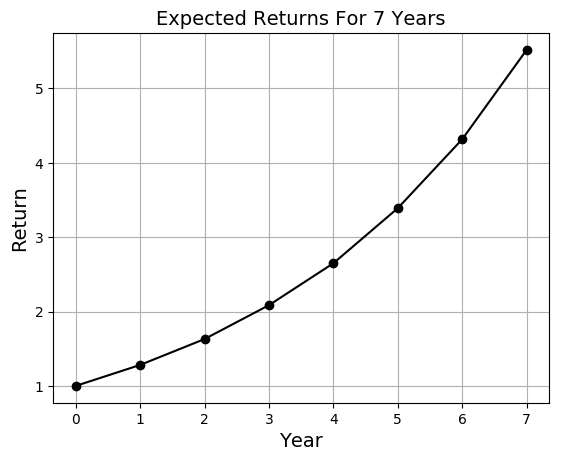
\includegraphics[width=.35\linewidth]{/app/plts/line.png}
  \end{tabular}
  \end{center}

  \begin{center}
      Prescribed Portfolio 1 Year Projections
      %(a) Returns of Current Portfolio
      %(a) Bell Curves Of Expected Return
  \end{center}

  \vspace{.7cm}


\begin{center}
  \begin{tabular}{lcr}
  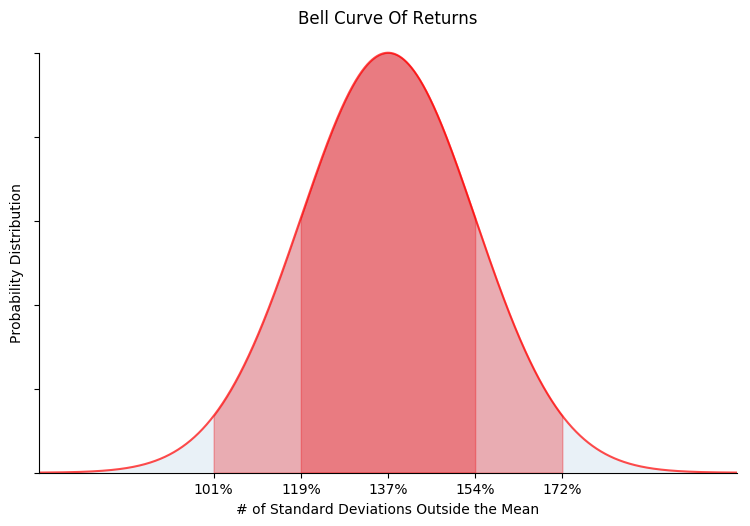
\includegraphics[width=.35\linewidth]{/app/plts/bell.png}
    & \hspace{1cm }&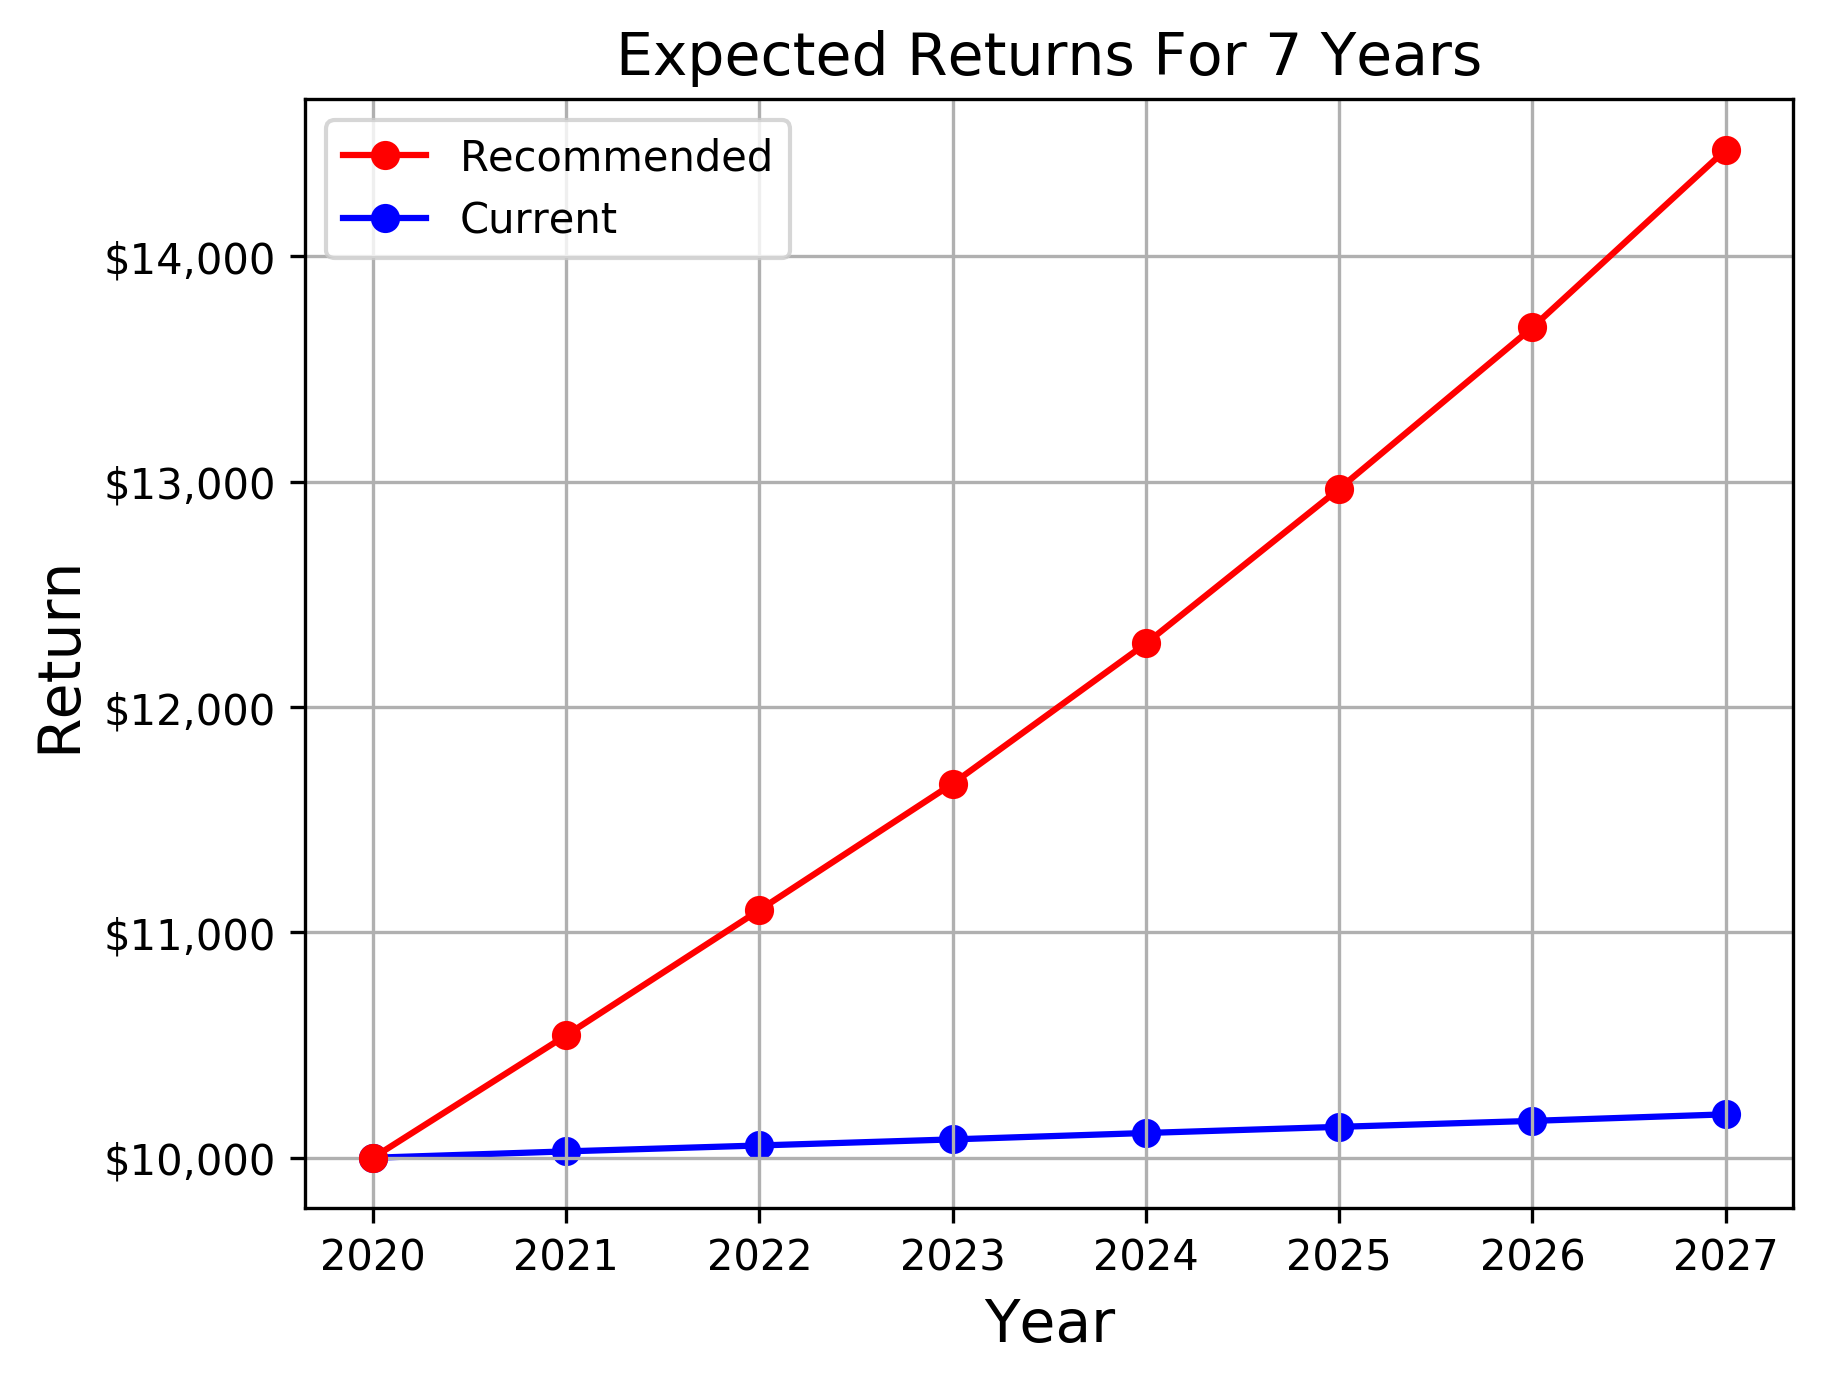
\includegraphics[width=.35\linewidth]{/app/plts/line7.png}
  \end{tabular}
  \end{center}

  \begin{center}
      Prescribed Portfolio 7 Year Projections
      %(a) Returns of Current Portfolio
      %(a) Bell Curves Of Expected Return
  \end{center}

\vspace{.6cm}

\end{adjustwidth}

\noindent
1 Year Expected Return (\$) : \$343,203.20 (33.3\%)\\
1 Year Risk (Standard Deviation \%) : $\pm$ 3.54\%

\noindent
7 Year Expected Return (\$) : \$343,203.20 (33.3\%)\\
7 Year Risk (Standard Deviation \%) : $\pm$ 3.54\%

\noindent
Sharpe Ratio : .37


\newpage



\section{Frontier Curve}

In 1990, Harry Markowitz won a nobel prize for his contributions to portfolio balancing theory. Markowitz discovered that given assets to buy from and funds to buy with, all of the optimal portfolios formed on a curved line called the "Frontier Curve."

\vspace{2cm}

\hspace*{-1cm}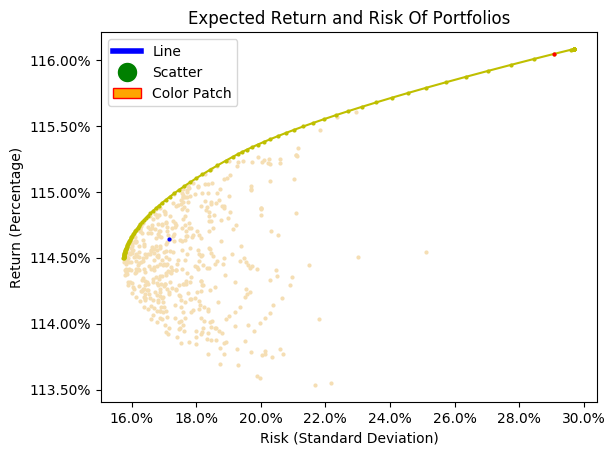
\includegraphics{/app/plts/frontier.png}\par

\vspace{1cm}


Risk (Std. Deviation) : $\pm$ {\VAR{risk_new}} \%

Expected Return (\%): {\VAR{ret_new}} \%

Improvement in risk : $\pm$ {\VAR{risk_improve}} \%

Improvement in return (\%): {\VAR{ret_improve}} \%


\newpage

\section{Correlation Matrices}

\vspace{1cm}

\begin{center}

\begin{tabular}{cccccccc} \toprule
    Corr. & MSFT & NTFX & HULU  & RUS & BP & TR & SOCK\\ \midrule
    MSFT  & 16.128 & +8.872 & 16.128 & 1.402 & 1.373 & -146.6 & -137.6 \\\midrule
    NTFX  & 3.442  & -2.509 & 3.442  & 0.299 & 0.343 & 133.2  & 152.4  \\\midrule
    HULU  & 1.826  & -0.363 & 1.826  & 0.159 & 0.119 & 168.5  & -161.1 \\\midrule
    RUS  & 0.993  & -0.429 & 0.993  & 0.086 & 0.08  & 25.6   & 90     \\ \midrule
    BP  & 1.29   & +0.099 & 1.29   & 0.112 & 0.097 & -175.6 & -114.7 \\\midrule
    TR  & 0.483  & -0.183 & 0.483  & 0.042 & 0.063 & 22.3   & 122.5  \\\midrule
    SOCK  & 0.766  & -0.475 & 0.766  & 0.067 & 0.039 & 141.6  & -122    \\ \bottomrule
\end{tabular}

\end{center}

Above is the Semantic Correlation Matrix of the selected Asset Classes. It shows how each asset class is correlated to one another

\vspace{1cm}



\begin{center}

\begin{tabular}{cccccccc} \toprule
    Return & MSFT & NTFX & HULU  & RUS & BP & TR & SOCK\\ \midrule
    1  & 16.128 & +8.872 & 16.128 & 1.402 & 1.373 & -146.6 & -137.6 \\
    2  & 3.442  & -2.509 & 3.442  & 0.299 & 0.343 & 133.2  & 152.4  \\

\end{tabular}

\end{center}


Above is the ranking of the selected asset classes by risk

\vspace{1cm}


\begin{center}

\begin{tabular}{cccccccc} \toprule
    Risk & MSFT & NTFX & HULU  & RUS & BP & TR & SOCK\\ \midrule
    1  & 16.128 & +8.872 & 16.128 & 1.402 & 1.373 & -146.6 & -137.6 \\
    2  & 3.442  & -2.509 & 3.442  & 0.299 & 0.343 & 133.2  & 152.4  \\

\end{tabular}

\end{center}


Above is the ranking of the selected asset classes by return


\medskip


%\printbibheading[heading=bibintoc,title={Bibliografia}]
%\bibbysection[heading=bibbysubsect]


\end{document}
